\documentclass{article}
\title{Mathematical Notes}
\author{Serafí Nebot Ginard}
\date{2023}

\usepackage[parfill]{parskip}
\usepackage{hyperref}
\usepackage{amsmath}
\usepackage{amssymb}
\usepackage{tikz}

\begin{document}
\maketitle
\newpage

\tableofcontents
\newpage

\section{Vectors}
\subsection{Definitions}
Vectors are ordered lists of numbers. Each component in a vector represents a dimension in space.
\[
	\vec{v} \in \mathbb{R}^n
\]
where $n$ indicates the dimension of a vector.

Vectors are denoted with square brackets with its values ordered from top to bottom
\[
	\vec{v} = \begin{bmatrix}
		v_1 \\
		v_2 \\
		\vdots \\
		v_n \\
	\end{bmatrix} \colon \{\vec{v} \in \mathbb{R}^n\}
\]

Points are denoted with parenthesis with its values ordered from left to\\right
\[
	p = \left(p_1, p_2, \dots, p_n \right)
\]

The transpose of a vector is a vector containing the values of the original vector as columns
\[
	\vec{v}^T = \begin{bmatrix}
		v_1, & v_2, & \dots, & v_n
	\end{bmatrix}
\]

\pagebreak
\subsection{Vector operations}
\subsubsection{Addition}
Addition is performed component by component
\begin{equation*}
	\begin{aligned}
		\vec{v} + \vec{w} &=
		\begin{bmatrix}
			1 \\
			2 \\
			4
		\end{bmatrix}
		+
		\begin{bmatrix}
			5 \\
			3 \\
			-2
		\end{bmatrix}
		\\
		\vec{v} + \vec{w} &=
		\begin{bmatrix}
			1 + 5 \\
			2 + 3 \\
			4 + (-2)
		\end{bmatrix}
		\\
		\vec{v} + \vec{w} &=
		\begin{bmatrix}
			6 \\
			5 \\
			2
		\end{bmatrix}
	\end{aligned}
\end{equation*}

In a coordinate system, vector addition is equivalent to moving the origin of one vector to the end
of the other. For example, given the following vectors
\begin{equation*}
	\begin{aligned}
		\vec{v} &=
		\begin{bmatrix}
			1 \\
			2
		\end{bmatrix},
		\vec{w} =
		\begin{bmatrix}
			-2 \\
			1
		\end{bmatrix}
		\\
		\vec{u} &= \vec{v} + \vec{w} =
		\begin{bmatrix}
			1 \\
			2
		\end{bmatrix}+
		\begin{bmatrix}
			-2 \\
			1
		\end{bmatrix} =
		\begin{bmatrix}
			-1 \\
			3
		\end{bmatrix}
	\end{aligned}
\end{equation*}
we may visualize them in a coordinate system
\begin{center}
	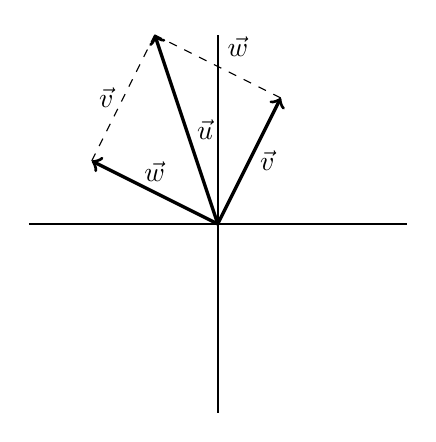
\begin{tikzpicture}[scale=0.8]
		\draw[thick] (-3, 0) -- (3, 0);
		\draw[thick] (0, -3) -- (0, 3);
		\draw[->, very thick] (0, 0) -- node[right] {$\vec{v}$} (1, 2);
		\draw[->, very thick] (0, 0) -- node[above] {$\vec{w}$} (-2, 1);
		\draw[-, dashed] (-2, 1) -- node[left] {$\vec{v}$} (-1, 3);
		\draw[-, dashed] (1, 2) -- node[above right] {$\vec{w}$} (-1, 3);
		\draw[->, very thick] (0, 0) -- node[right] {$\vec{u}$} (-1, 3);
	\end{tikzpicture}
\end{center}

\pagebreak
\subsubsection{Scalar multiplication}
Multiplication is performed by multiplying component of a vector by a scalar. For example:
\[
	\left\lbrace a = 2 \colon a \in \mathbb{R} \mid \vec{v} =
	\begin{bmatrix}
		3 \\
		2
	\end{bmatrix}
	\colon \vec{v} \in \mathbb{R}^2
	\right\rbrace
\]
\[
	a \times \vec{v} = 2 \times
	\begin{bmatrix}
		3 \\
		2
	\end{bmatrix}
	=
	\begin{bmatrix}
		6 \\
		4
	\end{bmatrix}
\]

Multiplying a vector by a scalar will "scale" the vector.
\begin{center}
	\begin{tikzpicture}
		\draw[-, thick] (-3, 0) -- (3, 0);
		\draw[-, thick] (0, -3) -- (0, 3);
		\draw[->, very thick] (0, 0) -- node[above] {$\vec{v}$} (1.5, 1);
		\draw[->, very thick, dashed] (1.5, 1) -- node[above left] {$2 \times \vec{v}$} (3, 2);
		\draw[->, very thick, dashed] (0, 0) -- node[above left] {$-1 \times \vec{v}$} (-1.5, -1);
	\end{tikzpicture}
\end{center}


\newpage
\subsection{Modulus}
The modulus of a vector is a number which determines the length of a vector in space. It is always
positive and does not indicate a direction. The modulus may be calculated as follows
\[
	|\vec{u}| = \sqrt{u_1^2 + u_2^2 + \dots + u_n^2}
\]

\subsection{Unit vector}
The unit vector, or normalized vector, is a vector whose modulus is equal to $1$. It is commonly denoted with a hat symbol on
top.
\[
	\left\lbrace \hat{u} =
		\begin{bmatrix}
			u_1 \\
			u_2 \\
			\dots \\
			u_n
		\end{bmatrix} \colon \hat{u} \in \mathbb{R}^n
	\right\rbrace
\]
\[
	|\hat{u}| = \sqrt{u_1^2 + u_2^2 + \dots + u_n^2} = 1
\]

The normalized vector $\hat{u}$ is the unit vector in the direction of $\vec{u}$
\[
	\hat{u} = \frac{\vec{u}}{|\vec{u}|}
\]

\newpage

\section{Trigonometry}
Let $\vec{u}_x$ be a vector on the horizontal axis, $\vec{u}_y$ a vector on the vertical axis,
$\vec{u}$ the linear combination of $\vec{u}_x$ and $\vec{u}_y$, and $\alpha$ the angle between the
horizontal axis and $\vec{u}$

\begin{center}
	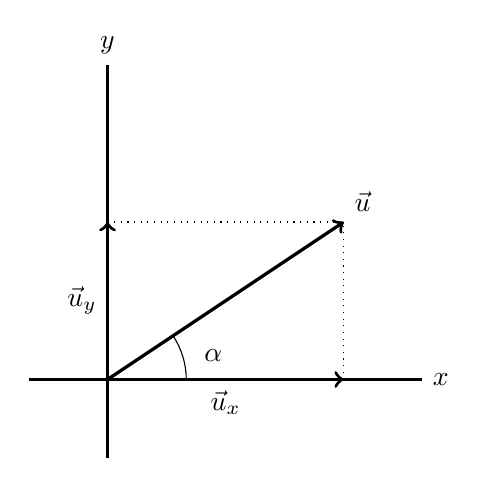
\begin{tikzpicture}
		\draw (1, 0) node[above right=3] {$\alpha$} arc[radius=1, start angle=0, end angle=acos(3/sqrt(3^2 + 2^2))] -- (0, 0) --
			cycle;
		\draw[-, thick] (-1, 0) -- (4, 0) node[right] {$x$};
		\draw[-, thick] (0, -1) -- (0, 4) node[above] {$y$};
		\draw[->, very thick] (0, 0) -- node[below] {$\vec{u}_x$} (3, 0);
		\draw[->, very thick] (0, 0) -- node[left] {$\vec{u}_y$} (0, 2);
		\draw[->, very thick] (0, 0) -- (3, 2) node[above right] {$\vec{u}$};
		\draw[-, dotted] (3, 0) -- (3, 2);
		\draw[-, dotted] (0, 2) -- (3, 2);
	\end{tikzpicture}
\end{center}

$\vec{u}$ may be calculated as the linear combination of $\vec{u}_x$ and $\vec{u}_y$
\[
	\vec{u} = \beta_x \vec{u}_x + \beta_y \vec{u}_y
\]
where $\beta_x$ and $\beta_y$ equal 1.

Considering the angle $\alpha$ we have that
\begin{equation*}
	\begin{aligned}
		\cos \alpha &= \frac{|\vec{u}_x|}{|\vec{u}|} \to |\vec{u}_x| = |\vec{u}| \cdot \cos \alpha
		\\ 
		\sin \alpha &= \frac{|\vec{u}_y|}{|\vec{u}|} \to |\vec{u}_y| = |\vec{u}| \cdot \sin \alpha
	\end{aligned}
\end{equation*}
therefore, $\alpha$ may be calculated from the given vectors
\begin{equation*}
	\begin{aligned}
		\alpha &= \cos^{-1}\frac{|\vec{u}_x|}{|\vec{u}|} \\
		\alpha &= \sin^{-1}\frac{|\vec{u}_y|}{|\vec{u}|}
	\end{aligned}
\end{equation*}

\end{document}
